\documentclass[a4paper,12pt]{article}
\usepackage[spanish]{babel}
\usepackage[utf8]{inputenc}
\usepackage{booktabs}
\usepackage{dirtytalk}
\usepackage{graphicx}
\usepackage{dirtytalk}
\usepackage[T1]{fontenc}
\usepackage[document]{ragged2e}
\usepackage{listings}

\begin{document}

\section{Código}

\begin{lstlisting}
library ieee;
use ieee.std_logic_1164.all;
use ieee.std_logic_arith.all;

entity Practica0 is port (
	a,b,ref : in std_logic_vector(2 downto 0);
	sel : in std_logic;
	display: out std_logic_vector(6 downto 0)
);
end Practica0; 

architecture aPractica0 of Practica0 is
signal aux, codigo : std_logic_vector (2 downto 0);
begin
	--mux
	aux <= a when sel = '0' else b;

	--comparador
	process (aux, ref)
	begin 
		if (aux < ref) then
			codigo <= "100";
		elsif (aux > ref) then 
			codigo <= "001";
	    else
			codigo <= "010";
		end if;
	end process;

	--decodificador
	process (codigo)
	begin 
		if (codigo = "001" ) then
			display <= "1111000";
		elsif (codigo = "100") then 
			display <= "1001110";
		elsif (codigo = "010") then
			display <= "1001000";
		else
			display <= "-------";
		end if;
	end process;

end aPractica0;
\end{lstlisting}

\section{Simulación}

\begin{figure}[h]
\centering
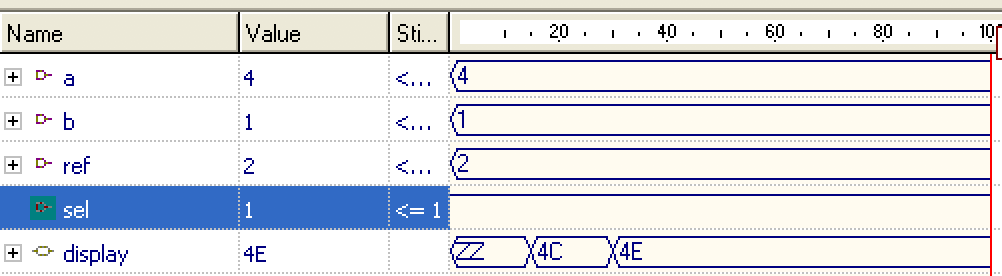
\includegraphics[scale=.5]{Menor1001110}
\caption{Display muestra menor.}
\end{figure}

\begin{figure}[h]
\centering
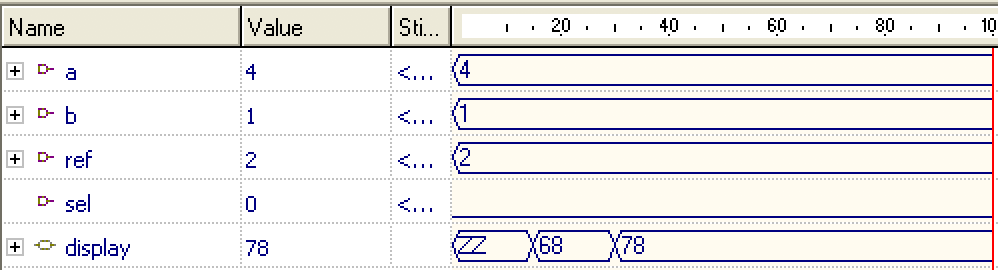
\includegraphics[scale=.5]{Mayor1111000}
\caption{Display muestra mayor.}
\end{figure}

\begin{figure}[h]
\centering
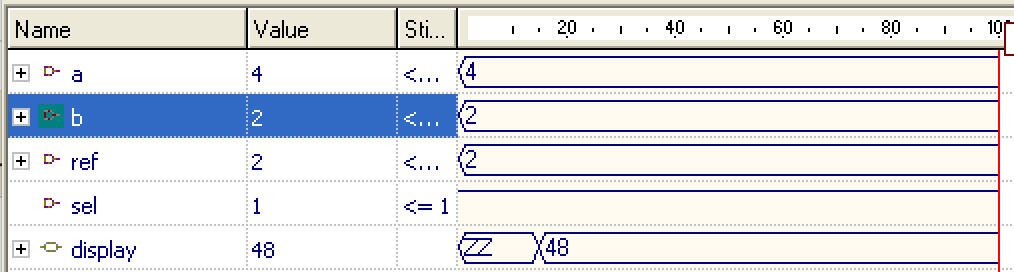
\includegraphics[scale=.5]{Igual1001000}
\caption{Display muestra igual.}
\end{figure}

\end{document}